\chapter{Introduzione}

\section{Intro al Corso}

\paragraph{Parole chiave:}

\begin{itemize}
  \item Web Apps. 
  \item Mission Critical.
  \item DevOps.
  \item Cloud Native.

\end{itemize}

\dfn{Mission Critical Applications}{
  Un'applicazione o sistema le cui operazioni sono fondamentali per una compagnia o un'istituzione.
}

\clm{}{}{
  \begin{itemize}
    \item Enfasi sui requisiti non funzionali: i requisiti funzionali sono la baseline, ma ci si aspetta di più per rimanere competitivi. 
    \item Da non confondere con life critical: non muore nessuno.
  \end{itemize}
}

\dfn{Enterprise Application Integration (EAI)}{
  Tutto l'insieme di pratiche architetturali, tecnologie, patterns, frameworks e strumenti che consentono la comunicazione e la condivisione tra diverse applicazioni nella stessa organizzazione.
}

\paragraph{Si ha enfasi sull'infrastruttura:} 
\begin{itemize}
  \item \fancyglitter{Data Integration:} combinare dati da più moduli diversi (coinvolge database). 
  \item \fancyglitter{Process Integration:} le interazioni tra più moduli. 
  \item \fancyglitter{Functional Integration:} si vuole fornire una nuova funzionalità sfruttando funzionalità già esistenti.
\end{itemize}
\pagebreak
\subsection{Esempio e Requisiti Non Funzionali}

\begin{figure}[h]
    \centering
    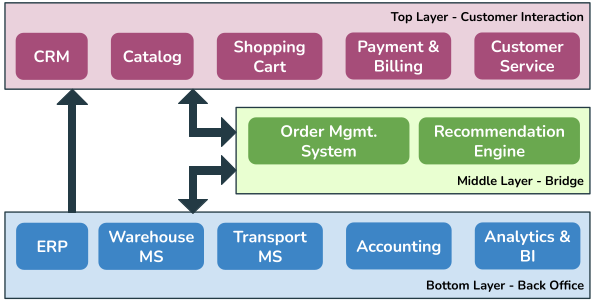
\includegraphics[scale=0.4]{01/crm.png}
    \caption{Esempio di e-commerce.}
\end{figure}

\paragraph{Commento dell'esempio:}

\begin{itemize}
  \item Ci sono tre livelli: 
    \begin{itemize}
      \item Top Layer: moduli che si rivolgono al cliente.
      \item Middle Layer: gestione della comunicazione tra cliente e azienda. 
      \item Bottom Layer: moduli interni aziendali.
    \end{itemize}
\end{itemize}

\paragraph{Requisiti non funzionali:}

\begin{itemize}
  \item High availability/zero downtime: l'applicativo deve essere sempre o quasi sempre disponibile. 
  \item Affidabilità: in caso di interruzione di workflow si deve far sì che non ci siano stati danni (e.g. un'interruzione durante una transazione). 
  \item Consistenza dei dati. 
  \item Integrità dei dati. 
  \item Low latency: per avere una buona performance, tutto deve essere fluido. 
  \item Scalabilità.
  \item Sicurezza. 
  \item Resilienza: capacità di reagire agli errori. 
  \item Mantenibilità: quanto un pezzo di software sia mantenibile o riutilizzabile.
  \item Osservabilità: per comprendere eventuali problemi in un sistema distribuito. 
  \item Auditability: le verifiche di qualità fatte su software\footnote{Meglio visto in "Etica, Società e Privacy".}.
\end{itemize}

\section{Panoramica Storica}

\subsection{Dagli Anni '70 al 2000}

\dfn{Waterfall}{
  Le metodologie a cascata\footnote{Viste a "Sviluppo delle Applicazioni Software".} sono metodologie in cui ci sono fasi ben distinte e separate tra loro.
}

\nt{È un modello prevedibile, ma lento a gestire i cambiamenti.}

\clm{}{}{
  \begin{itemize}
    \item Software on the shelf: una volta acquistato è proprio. 
    \item Software custom: prodotto su richiesta, ha bisogno di tutto un servizio di manutenzione. 
  \end{itemize}
}

\dfn{Lean}{
  Metodologie nate negli anni '50 alla Toyota, verranno applicate al software dagli anni '90. Si basa su tre principi: 
  \begin{itemize}
    \item Muda\footnote{JOJO'S Reference} (waste): si deve stare sui requisiti, non mettere troppe funzioni non necessarie. 
    \item Mura (unevenness): è necessaria consinstenza per aumentare la prevedibilità.  
    \item Muri (overburden): non sovraccaricare le persone o le macchine. Non progettare software utilizzando strumenti greedy di risorse.
  \end{itemize} 
}

\nt{Lo strumento fondamentale è il \fancyglitter{kanban}: la lavagna, per organizzare il lavoro.}

\dfn{Siloed}{
  Organizzazione aziendale a silos: si comunica poco e male. Ci sono 4 gruppi: 
  \begin{itemize}
    \item BA Team: relazioni con gli stakeholders, requisiti, specifiche, documentazione. 
    \item Dev Team: programma e fa un minimo di unit testing. 
    \item Test Team: testa e decide se il sistema è pronto. 
    \item Ops Team: si occupa del deployement.
  \end{itemize}
}

\nt{I vari team si parlano in maniera molto limitata.}

\dfn{Transaction Processing Monitor}{
  I TP monitor erano il primo esempio di soluzione middleware. Usata nei sistemi di mainframe erano: centralizzati, monolitici, mission critical, con accesso da vari terminali.
}

\cor{Middleware}{
  Software nel mezzo tra applicazioni e infrastrutture. Permette alle applicazioni di utilizzare le infrastrutture per farle comunicare tra di loro.
}

\paragraph{Obiettivi:}

\begin{itemize}
  \item Performance: si occupa di transazioni rispettando le proprietà ACID. 
  \item Scalabilità: se un programma crasha ne avvia un'altra istanza. 
  \item Affidabilità. 
  \item Consistenza dei dati.
\end{itemize}

\paragraph{Limiti:}

\begin{itemize}
  \item Proprietario. 
  \item Tight coupling. 
  \item Costosi. 
  \item Complessi.
\end{itemize}

\qs{}{Cosa rimane dei TP monitors?}

\begin{itemize}
  \item \fancyglitter{Gestione delle transazioni e coordinazione:}
    \begin{itemize}
      \item Soluzioni basate su 2PC (2 Phase Commit). 
      \item Le proprietà ACID, attualmente supportate internamente da molti database. 
      \item Proprietà BASE: 
        \begin{itemize}
          \item Basically: risposte basiche.
          \item Available: si accetta che si possa non avere il dato più aggiornato. 
          \item State: la consistenza potrebbe non essere rispettata.
          \item Eventually: prima o poi si riceverà il dato corretto.
        \end{itemize}
    \end{itemize}
  \item \fancyglitter{Pool di connessioni}. 
  \item \fancyglitter{Distribuzione del carico:}
    \begin{itemize}
      \item Le richieste vengono distribuite su varie istanze. 
      \item In caso di fallimento l'applicazione riparte.
    \end{itemize}
\end{itemize}

\dfn{Remote Procedure Call}{
  Si chiama una funzione da una macchina remota come se fosse locale. È indipendente dal linguaggio e a una struttura silos. RIchiede aggiunte sia nello sviluppo che a runtime.
}

\begin{figure}[h]
    \centering
    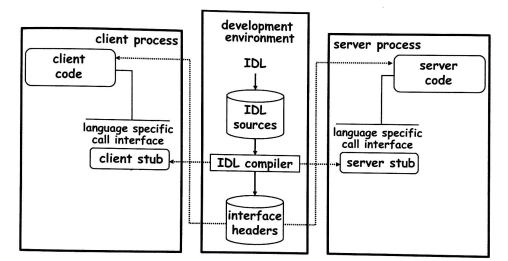
\includegraphics[scale=0.55]{01/rpc1.png}
    \caption{Remote Procedure Call - Development.}
\end{figure}

\begin{itemize}
  \item Serializzazione: trasformare i dati in qualcosa che può essere comunicato.
  \item Marshalling: usa la serializzazione e inserisce meta-dati per permettere la ricostruzione della struttura dati.
\end{itemize}

\begin{figure}[h]
    \centering
    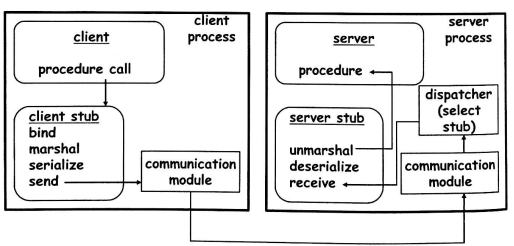
\includegraphics[scale=0.55]{01/rpc2.png}
    \caption{Remote Procedure Call - Runtime.}
\end{figure}

\dfn{Common Object Request Broker Architecture (CORBA)}{
  Evoluzione di rpc pensata per gli oggetti. Si possono creare oggetti in un server che possono rispondere a chiamate remote.
}

\nt{Più successo lo ha avuto RMI (Remote Method Invocation) che è CORBA, ma solo con Java.}

\paragraph{Limiti:}

\begin{itemize}
  \item Nascondere le cose al programmatore: si ha un falso senso di disaccoppiamento e i programmatori tendono a non vedere la rete. 
  \item La programmazione sembra semplice perché i problemi vengono sottovalutati.
\end{itemize}

\dfn{Message Oriented Middleware}{
  Invece di chiamarsi a vicenda le applicazioni si inviano messaggi a vicenda:
  \begin{itemize}
    \item Sincronizzazione tra operazioni in applicazioni diverse. 
    \item Notifiche di eventi. 
    \item Non c'è necessità di conoscere il ricevente.
  \end{itemize}
}

\paragraph{Due modelli di comunicazione:}

\begin{itemize}
  \item Point-to-Point: il mittente manda un messaggio nella coda del middleware, il ricevente lo consuma. 
  \item Publish and Subscribe: c'è una bacheca su cui chiunque può pubblicare un evento.
\end{itemize}

\dfn{Enterprise Service Bus (ESB)}{
  Un middleware coscente della logica di business. Si occupa di tradurre protocolli e dati.
}

\nt{Caduto totalmente in disuso.}

\subsection{Dal 2000 ai Giorni Nostri}

\dfn{AGILE}{
  Metodologie fondate su itertività e incrementalità.
}

\cor{XP - Xtreme Programming}{
  Si concentra sul codice, lo sviluppo di software si fa in team. Si dà importanza ai feedback sia dai clienti che dagli sviluppatori (small release, test-driven development, on-site customer).
}

\paragraph{Principi di XP:}

\begin{itemize}
  \item Comunicazione. 
  \item Semplicità. 
  \item Feedback. 
  \item Coraggio. 
  \item Rispetto.
\end{itemize}

\dfn{Scrum}{
  Prassi di organizzazione dell'attività lavorativa degli sviluppatori, si concentra sulla comunicazione:
  \begin{itemize}
    \item Organizzazione: esiste una lista del lavoro che deve essere svolto (Product Backlog e PDI), un'iterazione di lavoro di massimo 4 settimane (sprint) e deve esserci un incremento (valore percepibile dal cliente).
    \item Ruoli: ci si organizza in piccoli teams per ogni modulo.
  \end{itemize}
}

\paragraph{Ruoli in Scrum:}

\begin{itemize}
  \item Product owner: persona che gestisce il Backlog, in contatto con i clienti (non è il capo). 
  \item Scrum master: organizza le riunioni, fa da mediatore. 
  \item Development team.
\end{itemize}

\paragraph{Eventi per ogni sprint:}

\begin{itemize}
  \item Sprint panning: riunione in cui si decide cosa fare.
  \item Daily scrum: meeting in piedi, deve durare poco.
  \item Sprint review: alla fine dello sprint, si mostra l'incremento agli stakeholders.
  \item Sprint retrocspective: dopo la review, è una riunione interna al team.
\end{itemize}

\dfn{Kanban}{
  Si vuole mantenere il flusso di lavoro. Non si mette più lavoro di quello che si riesce a fare.
}

\paragraph{Principi di Kanban:}

\begin{itemize}
  \item Visualizzazione: si vede il proprio lavoro attraverso delle lavagne su cui vengono appiccicati post-it.
  \item WIP limit: si fanno un certo numero di cose contemporaneamente (non più di 3-4). 
  \item Pull system\footnote{Gacha moment.}: le cose vengono spostate dal to do al doing quando si libera un posto. 
  \item Continuous delivery: si integra la feature implementata e la si consegna. 
\end{itemize}

\paragraph{Board:}

\begin{itemize}
  \item Backlog. 
  \item To do: roba da fare. 
  \item Doing (WIP limit): roba che si sta facendo. 
  \item Done: roba fatta.
\end{itemize}

\dfn{Scrumban}{
  Scrum: ha i ruoli, il product Backlog e PBI, daily meeting, sprints. 

  Kanban: il flusso è pull-based e usa i WIP limit, le lavagne e i Continuous
   delivery.
}

\paragraph{Siloed evoluta:}

\begin{itemize}
  \item Biz team: relazioni con gli stakeholders, marketing e vendite. 
  \item Dev team: requisiti, sviluppo, testing e comunicazione con il biz team. 
  \item Ops team: deploy, setting, validazioni.
\end{itemize}

\nt{La divisione c'è ancora, ma c'è più comunicazione tra i vari team.}

\dfn{Service-Oriented Architecture}{
  Si inizia a ragionare sul fatto che l'integrazione debba avvenire mediante moduli che forniscono servizi l'uno all'altro.
}

\qs{}{Cos'è un servizio?}

\cor{Servizio}{
  Un servizio è una capacità di business autocontenuta che viene esposta secondo un contratto standard (un'interfaccia).
}

\paragraph{I servizi:}

\begin{itemize}
  \item \fancyglitter{Coarse-grained:} ogni servizo implementa tutto (più pesanti dei microservizi). 
  \item Condivide dati e funzioni attraverso interfacce (o API). 
  \item \fancyglitter{Scopribili:} i servizi si scoprono attraverso nomi e non IP.
\end{itemize}

\paragraph{SOA:}

\begin{itemize}
  \item Comunicazione attraverso applicazioni apposta o protocolli basati su HTTP. 
  \item Le infrastrutture hanno un ruolo importante nel comporre i servizi in funzioni. 
  \item Deployment centralizzato.
\end{itemize}

\dfn{Web Services}{
  Istanza di Service-Oriented Architecture che stabilisce:
  \begin{itemize}
    \item Protocollo di comunicazione (SOAP):
      \begin{itemize}
        \item XML su HTTP. 
        \item Consente sia comunicazione sincrona che asincrona.
      \end{itemize}
    \item Service registry: UDDI
      \begin{itemize}
        \item Elenco di servizi registrati secondo le loro features generali. 
        \item Consente ai servizi di essere scopribili. 
        \item Comunicazione mediante SOAP.
      \end{itemize}
    \item Contratto (WSDL, Web Service Description Language): 
      \begin{itemize}
        \item Fornisce informazioni per contattare effettivamente un servizio. 
        \item La struttura dei messaggi. 
        \item Le strutture dati. 
        \item Protocollo e indirizzo.
      \end{itemize}
  \end{itemize}
}

\clm{Sui Web Services}{}{
  Idealmente:
  \begin{itemize}
    \item Il client cerca il servizio su UDDI. 
    \item Ottiene il link dal WSDL del servizio. 
    \item Utilizzando WSDL collega dinamicamente il servizio alle operazioni.
  \end{itemize}
  In Pratica:
  \begin{itemize}
    \item La scoperta di servizi "in tempo reale"  era impraticabile. 
    \item I WSDL erano in maggioranza statici. 
    \item Le informazioni venivano salvate in file di configurazione.
  \end{itemize}
}

\subsection{JavaEE e Cloud}

\dfn{Enterprise Java Beans (EJB)}{
 Gli EJB sono oggetti resi disponibili dinamicamente. Offrivano:
 \begin{itemize}
\item Gestione del lifecycle. 
  \item RMI. 
  \item Sicurezza basata sui ruoli. 
  \item Persistenza tramite Object-relational mapping (ORM). 
  \item Gestione delle transazioni ACID.
 \end{itemize}
}

\paragraph{I Java Beans erano pesanti:}

\begin{itemize}
  \item Oggetti collegati alla JVM (al container). 
  \item Molto accoppiati all'ambiente di esecuzione. 
  \item Necessitavano un java application server. 
  \item Molto codice boiler-plate. 
  \item Annotazioni XML. 
  \item Non portabili.
\end{itemize}

\nt{Tutto questo fino al 2006 in cui la terza edizione di EJB li fa diventare più leggeri:
\begin{itemize}
  \item Annotazioni Java al posto di XML.
  \item POJOs (Plain Old Java Objects). 
  \item JPA (Java Persistence). 
  \item Si integrano con web service. 
  \item Introduzione della \fancyglitter{dependency injection}: design pattern per collegare due o più moduli tramite l'ambiente di sviluppo stesso.
\end{itemize}
}

\dfn{Cloud}{
  Insieme di risorse sia comptazionali, sia di storage, sia di networking. Queste risorse sono rese disponibili come servizi mediante API.
}

\clm{}{}{
  \begin{itemize}
    \item Il cloud è un'astrazione che nasconde la struttura fisica delle macchine. 
    \item C'è un livello simile a un OS. 
    \item I servizi sono offerti su base dichiarativa: diventa possibile avere un servizio che si conformi alle proprie necessità.
  \end{itemize}
}

\paragraph{Modelli:}

\begin{itemize}
  \item \fancyglitter{Infrastructure as a Service (IaaS):} l'azienda mette a disposizione macchine virtuali, di storage o sottoreti visibili a chi compra il servizio. 
  \item \fancyglitter{Platform as a Service (PaaS):} si acquista una piattaforma che nasconde cose e ottimizza. 
  \item \fancyglitter{Function as a Service (FaaS):} si carica su una piattaforma una serie di funzioni e si sviluppa solo il front end.
\end{itemize}

\paragraph{Applicazioni native sul cloud:}

\begin{itemize}
  \item Moduli molto leggeri e loosely-coupled. 
  \item Deployment contenerizzato (impacchettato e Platform independent), orchestrazione (ignorante rispettto all'architettura ma che può operare su essa) e elasting scaling (cambiare il livello dei servizi). 
  \item Dev Cycle features: integrazione continua, continuous delivery, deploy, infrastrutture dichiarative, consistenza tra dev/test/prod, anticipare i test sulla sicurezza, l'applicazione deve essere osservabile. 
  \item NFRs: scalabilità, portabilità, sicurezza, evoluzione, mantenibilità, affidabilità.
\end{itemize}

\dfn{DevOPs}{
  Gestione del sistema mediante l'utilizzo di tools e pratiche basato sui principi Lean.
}

\section{Ripasso su Spring Boot}

\nt{DISCLAIMER: è il mio primo approccio alla programmazione web (dato che sono specializzata in robe teoriche e/o a basso livello) per cui potrei fare qualche imprecisione, sorry.}

\subsection{Maven}

Dato che gli IDE moderni consumano un sacco di batteria e risorse includo anche una mini guida per setuppare un progetto java con Maven (in questo modo potete usare vim, gedit o nano se vi va). Se usate Intell*J, Vs C*de o altro potete saltare\footnote{Questi IDE possono utilizzare anche Maven, ma lo gestiscono loro.}.

\dfn{Maven}{
  Maven è un tool per creare automaticamente delle build di progetti java. Permette di compilare codice, fare testing, packaging, etc.
}

\nt{Maven utilizza il \fancyglitter{Project Object Model (POM)} per descrivere la configurazione di un progetto e gestire le dipendenze.}

\qs{}{Come si crea un progetto con Maven?}

\begin{lstlisting}[language=bash, caption={Creazione di un progetto Maven}]
mvn archetype:generate \
    -DgroupId=com.example \
    -DartifactId=myapp \
    -DarchetypeArtifactId=maven-archetype-quickstart \
    -DinteractiveMode=false
\end{lstlisting}

\paragraph{Nello specifico:}

\begin{itemize}
  \item \texttt{DgroupID} indica il nome di una compagnia o di un'organizzazione. 
  \item \texttt{DartifactId} indica il nome del progetto. 
  \item \texttt{DarchetypeArtifactId} indica il template (in questo caso un semplice HelloWorld java).
\end{itemize}

\paragraph{Per renderlo un progetto Spring Boot è necessario apportare le seguenti modifiche al \texttt{pom.xml}:}

\begin{lstlisting}[language=xml, caption={Esempio di pom.xml per Spring Boot}]
<project xmlns="http://maven.apache.org/POM/4.0.0"
         xmlns:xsi="http://www.w3.org/2001/XMLSchema-instance"
         xsi:schemaLocation="http://maven.apache.org/POM/4.0.0
         http://maven.apache.org/xsd/maven-4.0.0.xsd">
    <modelVersion>4.0.0</modelVersion>

    <parent>
        <groupId>org.springframework.boot</groupId>
        <artifactId>spring-boot-starter-parent</artifactId>
        <version>3.3.4</version>
        <relativePath/>
    </parent>

    <groupId>com.example</groupId>
    <artifactId>myapp</artifactId>
    <version>1.0.0-SNAPSHOT</version>
    <packaging>jar</packaging>
    <name>myapp</name>

    <properties>
        <java.version>24</java.version>
    </properties>

    <dependencies>
        <dependency>
            <groupId>org.springframework.boot</groupId>
            <artifactId>spring-boot-starter-web</artifactId>
        </dependency>
        <dependency>
            <groupId>org.springframework.boot</groupId>
            <artifactId>spring-boot-starter-test</artifactId>
            <scope>test</scope>
        </dependency>
    </dependencies>

    <build>
        <plugins>
            <plugin>
                <groupId>org.springframework.boot</groupId>
                <artifactId>spring-boot-maven-plugin</artifactId>
            </plugin>
        </plugins>
    </build>
</project>
\end{lstlisting}
\paragraph{Spiegazione:}
\begin{itemize}
  \item Il \texttt{parent} imposta la versione di Spring Boot e le configurazioni di default.
  \item Le \texttt{dependencies} includono il modulo web e quello per i test.
  \item Il plugin \texttt{spring-boot-maven-plugin} permette di eseguire l'app con \texttt{mvn spring-boot:run}.
\end{itemize}
\subsection{Gradle}

Per alcune persone può essere più facile utilizzare Gradle (inclusa me), quindi aggiungo qualcosa anche per questo. 

\dfn{Gradle}{
Come Maven, Gradle è un tool per creare automaticamente progetti java, C/C++, kotlin, etc. A livello di base ha le stesse funzionalità di Maven, le differenze principali sono il linguaggio utilizzato (Maven è basato su xml, Gradle su Groovy), velocità (Gradle è più veloce per build incrementali), etc.
}

\qs{}{Come si crea un progetto Spring Boot con Gradle?}

\begin{lstlisting}[language=bash, caption={Creazione di un progetto Spring Boot con Gradle}]
curl https://start.spring.io/starter.tgz \
         -d type=gradle-project \
         -d dependencies=web \
         -d groupId=com.example \
         -d artifactId=test \
         -d name=test \
         -d packageName=com.example.test \
         -o test-gradle.tgz
   tar -xvf test-gradle.tgz
   cd test
\end{lstlisting}

\paragraph{Alcune osservazioni importanti:}

\begin{itemize}
\item Di default il progetto creato usa java 17, per cambiarlo basta andare nel file \texttt{build.gradle}.
\item Inizialmente darà errore perché non si sono definiti endpoint.
\end{itemize}

\paragraph{Esecuzione del progetto:}

\begin{lstlisting}[language=bash, caption={Avvio del progetto Spring Boot con Gradle}]
# Su Linux/macOS
./gradlew bootRun

# Su Windows
gradlew.bat bootRun
\end{lstlisting}

\nt{Al primo avvio Gradle scaricherà tutte le dipendenze necessarie. Una volta completato, l'app sarà disponibile su \texttt{http://localhost:8080/}.  
Se non hai ancora definito controller o endpoint, vedrai la \textit{Whitelabel Error Page}.}

\subsection{Spring Boot}







